\documentclass[tikz,border=3pt]{standalone}
\ifdefined\pdfinfoomitdate
  \pdfinfoomitdate=1
\fi
\ifdefined\pdftrailerid
  \pdftrailerid{}
\fi
\ifdefined\pdfsuppressptexinfo
  \pdfsuppressptexinfo=15
\fi
\usepackage{amsmath,amssymb}
\usepackage{braket}
\usetikzlibrary{arrows.meta,backgrounds,calc,decorations.pathreplacing}
\definecolor{walkc}{HTML}{3B7DB3}
\definecolor{gqspc}{HTML}{7E5DA8}
\definecolor{selc}{HTML}{C79445}
\definecolor{fpaac}{HTML}{C06267}
\begin{document}
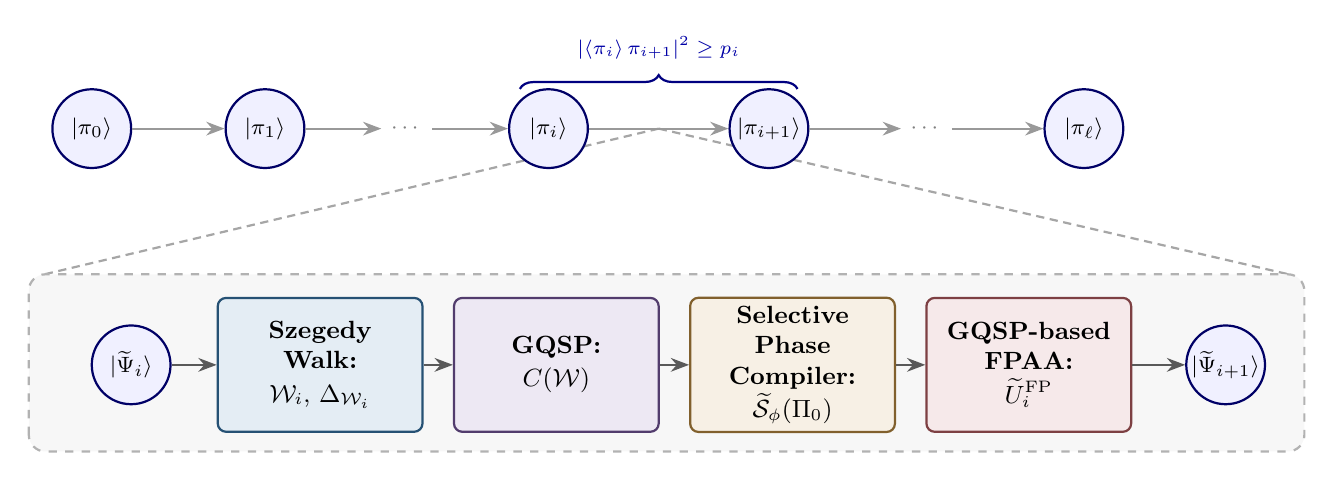
\begin{tikzpicture}[
    >=Stealth,
    font=\small,
    box/.style={
        draw=#1!65!black, thick, rounded corners=3pt,
        fill=#1!14, align=center,
        minimum height=17mm, minimum width=26mm,
        text width=23mm, inner sep=3pt},
    walk/.style={box=walkc},
    gqsp/.style={box=gqspc},
    sel/.style={box=selc},
    fpaa/.style={box=fpaac},
    sn/.style={
        circle, draw=blue!40!black, thick,
        fill=blue!6, inner sep=0pt,
        font=\footnotesize, minimum size=10mm},
]
% TOP ROW
\node[sn]   (p0)  at (0,    4.4) {$\ket{\pi_0}$};
\node[sn]   (p1)  at (2.2,  4.4) {$\ket{\pi_1}$};
\node[font=\footnotesize, text=black!50] (d1)  at (4.0,  4.4) {$\cdots$};
\node[sn]   (pi)  at (5.8,  4.4) {$\ket{\pi_i}$};
\node[sn]   (pi1) at (8.6,  4.4) {$\ket{\pi_{i+1}}$};
\node[font=\footnotesize, text=black!50] (d2)  at (10.6, 4.4) {$\cdots$};
\node[sn]   (pl)  at (12.6, 4.4) {$\ket{\pi_\ell}$};

\foreach \a/\b in {p0/p1, p1/d1, d1/pi, pi/pi1, pi1/d2, d2/pl}{
    \draw[->, thick, black!40] (\a) -- (\b);
}

\draw[decorate, decoration={brace, amplitude=5pt, raise=4pt},
      thick, blue!50!black]
    (pi.north west) -- (pi1.north east)
    node[midway, above=11pt, font=\scriptsize, text=blue!65!black]
    {$\lvert\braket{\pi_i}{\pi_{i+1}}\rvert^2 \ge p_i$};

\coordinate (arrowmid) at ($(pi.east)!0.5!(pi1.west)$);

\begin{scope}[on background layer]
\draw[thick, black!35, densely dashed] (arrowmid) -- (-0.6, 2.55);
\draw[thick, black!35, densely dashed] (arrowmid) -- (15.2, 2.55);
\end{scope}

% BOTTOM ROW
\begin{scope}[on background layer]
\fill[black!3, rounded corners=6pt] (-0.8, 0.3) rectangle (15.4, 2.55);
\draw[black!30, thick, rounded corners=6pt, dashed]
    (-0.8, 0.3) rectangle (15.4, 2.55);
\end{scope}

\node[sn]       (in)   at (0.5,  1.4) {$\ket{\widetilde{\Psi}_i}$};
\node[walk]     (s1)   at (2.9,  1.4) {\textbf{Szegedy Walk:}\\[1pt]$\mathcal{W}_i,\,\Delta_{\mathcal{W}_i}$};
\node[gqsp]     (s2)   at (5.9,  1.4) {\textbf{GQSP:}\\[1pt]$C(\mathcal{W})$};
\node[sel]      (s3)   at (8.9,  1.4) {\textbf{Selective Phase}\\\textbf{Compiler:}\\[1pt]$\widetilde{\mathcal{S}}_\phi(\Pi_{0})$};
\node[fpaa]     (s4)   at (11.9, 1.4) {\textbf{GQSP-based}\\\textbf{FPAA:}\\[1pt]$\widetilde{U}_i^{\mathrm{FP}}$};
\node[sn]       (out)  at (14.4, 1.4) {$\ket{\widetilde{\Psi}_{i+1}}$};

\foreach \a/\b in {in/s1, s1/s2, s2/s3, s3/s4, s4/out}{
    \draw[->, thick, black!65] (\a.east) -- (\b.west);
}
\end{tikzpicture}
\end{document}
